\documentclass[tikz, border=10pt]{standalone}
\usepackage{tikz}
\usetikzlibrary{shapes, positioning, arrows.meta, calc, backgrounds}

\begin{document}
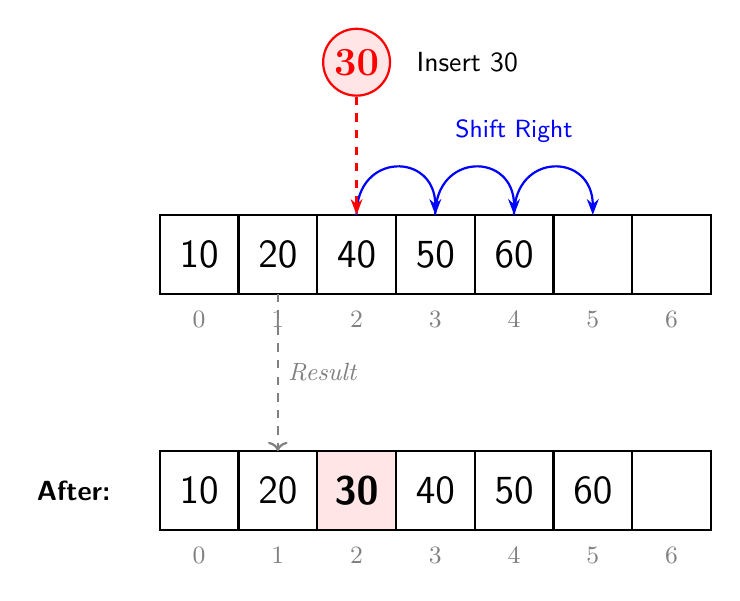
\begin{tikzpicture}[
    cell/.style={
        rectangle, 
        draw=black, 
        thick, 
        minimum width=1cm, 
        minimum height=1cm, 
        node distance=0cm, 
        outer sep=0pt,
        font=\Large\sffamily
    },
    index/.style={
        font=\small\ttfamily\color{gray},
        below=0.1cm of #1
    },
    arrow/.style={
        ->, 
        thick, 
        color=blue, 
        >={Stealth[length=2mm]}
    },
    newval/.style={
        circle,
        draw=red, 
        thick,
        fill=red!10,
        inner sep=2pt,
        minimum size=0.8cm,
        font=\Large\bfseries\color{red}
    }
]

    % Array cells
    \node[cell] (c0) {10};
    \node[cell, right=of c0] (c1) {20};
    \node[cell, right=of c1] (c2) {40};
    \node[cell, right=of c2] (c3) {50};
    \node[cell, right=of c3] (c4) {60};
    \node[cell, right=of c4] (c5) {}; % Empty slot
    \node[cell, right=of c5] (c6) {}; % Empty slot

    % Indices
    \node[below=0.1cm of c0, font=\small\color{gray}] {0};
    \node[below=0.1cm of c1, font=\small\color{gray}] {1};
    \node[below=0.1cm of c2, font=\small\color{gray}] (idx2) {2};
    \node[below=0.1cm of c3, font=\small\color{gray}] {3};
    \node[below=0.1cm of c4, font=\small\color{gray}] {4};
    \node[below=0.1cm of c5, font=\small\color{gray}] {5};
    \node[below=0.1cm of c6, font=\small\color{gray}] {6};

    % Highlighting the insertion point (index 2)
    \node[newval, above=1.5cm of c2] (new) {30};
    \node[right=0.2cm of new, font=\sffamily\color{black}] {Insert 30};

    % Arrows showing shifts
    % Shift 60 to 5
    \draw[arrow] (c4.north) .. controls +(up:0.8cm) and +(up:0.8cm) .. (c5.north);
    % Shift 50 to 4
    \draw[arrow] (c3.north) .. controls +(up:0.8cm) and +(up:0.8cm) .. (c4.north);
    % Shift 40 to 3
    \draw[arrow] (c2.north) .. controls +(up:0.8cm) and +(up:0.8cm) .. (c3.north);

    % Arrow for insertion
    \draw[arrow, color=red, dashed] (new.south) -- (c2.north);

    % Label for shift operation
    \node[above=0.8cm of c4, font=\small\sffamily\color{blue}] {Shift Right};

    % -- Final State --
    \node[below=2.0cm of c0, cell] (f0) {10};
    \node[below=0.1cm of f0, font=\small\color{gray}] {0};

    \node[cell, right=of f0] (f1) {20};
    \node[below=0.1cm of f1, font=\small\color{gray}] {1};

    \node[cell, right=of f1, fill=red!10] (f2) {\textbf{30}};
    \node[below=0.1cm of f2, font=\small\color{gray}] {2};

    \node[cell, right=of f2] (f3) {40};
    \node[below=0.1cm of f3, font=\small\color{gray}] {3};

    \node[cell, right=of f3] (f4) {50};
    \node[below=0.1cm of f4, font=\small\color{gray}] {4};

    \node[cell, right=of f4] (f5) {60};
    \node[below=0.1cm of f5, font=\small\color{gray}] {5};

    \node[cell, right=of f5] (f6) {};
    \node[below=0.1cm of f6, font=\small\color{gray}] {6};

    \node[left=0.5cm of f0, font=\sffamily\bfseries] {After:};

    % Arrow connecting states
    \draw[transform canvas={xshift=-2cm}, ->, thick, gray, dashed] ($(c0.south west)!0.5!(c6.south east)$) -- node[midway, right, font=\small\itshape] {Result} ($(f0.north west)!0.5!(f6.north east)$);

\end{tikzpicture}
\end{document}
